\section{Introductie}



\subsection{Projectbeschrijving}
\subsubsection{Doel en objectieven}

Dit project heeft als doel een webtoepassing te creëren waar men publicaties op kan plaatsen en beheren.  Het project is onderdeel van het vak Software Engineering dat gegeven wordt door Ragnhild Van Der Straeten \cite{rvdstrae} aan de Vrije Universiteit Brussel. De vereisten die gegeven zijn voor dit project, worden beschreven in het SRS.

\subsubsection{Veronderstellingen en beperkingen}
\paragraph{Veronderstellingen}
We gaan er van uit dat de toepassing op verschillende toestellen gaat werken, zodat mensen overal aan publicaties kunnen geraken. Na deze iteratie werkt de toepassing enkel nog maar op een computer maar in latere iteraties zal hier aan worden gewerkt.

\paragraph{Beperkingen}
\begin{itemize}
\item Het systeem moet werken onder Wilma \cite{Wilma} en een up-to-date browser. %LINK wilma
\item GitHub \cite{GitHub} moet gebruikt worden als repository.
\item Enkel JavaScript, HTML5, CSS en bijbehorende open-source frameworks en bibliotheken mogen worden gebruikt als programmeertaal of technologie.
\item Enkel vrije software mag gebruikt worden, zowel voor het eindproduct als voor hulpmiddelen.
\item Het systeem moet eenvoudig kunnen ge\"installeerd worden, op een standaard manier.
\item De grafische gebruikersinterface moet aantrekkelijk en eenvoudig zijn.
\end{itemize}

\subsubsection{Project Deliverables}

In onderstaande tabellen staan de data wanneer de documenten \ref{tab:doc} en de code \ref{tab:code} worden afgeleverd en wanneer presentaties \ref{tab:pres} over het project worden gegeven. 

\begin{table}[h]
\begin{minipage}[b]{0.45\linewidth}
\begin{tabularx}{1.9\textwidth}{c|c}
\hline
\textbf{Datum} & \textbf{Documenten}\\
 \hline
 Woensdag 05/11/2014 & inleveren SPMP \\
 Woensdag 19/11/2014 & eerste versie documenten \\
 Maandag 15/12/2014 & Einde iteratie 1: opleveren documenten \\
 \hline \hline
 Dinsdag 03/03/2015 & Einde iteratie 2: opleveren documenten \\
 Maandag 20/04/2015 & Einde iteratie 3: opleveren documenten \\
 Vrijdag 15/05/2015 & Einde iteratie 4: finale oplevering
\end{tabularx}
\caption{Documenten}
\label{tab:doc}
\end{minipage}

\vspace{0.5cm}

\begin{minipage}[b]{0.45\linewidth}
\begin{tabularx}{1.9\textwidth}{c|c}
\hline
\textbf{Datum} & \textbf{Code}\\
 \hline
 Maandag 15/12/2014 & Einde iteratie 1: opleveren code \\
 \hline \hline
 Dinsdag 03/03/2015 & Einde iteratie 2: opleveren code \\
 Maandag 20/04/2015 & Einde iteratie 3: opleveren code \\
 Vrijdag 15/05/2015 & Einde iteratie 4: finale oplevering
\end{tabularx}
\caption{Code}
\label{tab:code}
\end{minipage}
\vspace{0.5cm}

\begin{minipage}[b]{0.45\linewidth}
\begin{tabularx}{1.9\textwidth}{c|c}
\hline
\textbf{Datum} & \textbf{Presentaties}\\
 \hline
 Vrijdag 19/12/2014 & presentatie 1 \\
 \hline \hline
Woensdag 11/03/2015 & presentatie 2\\
Woensdag 22/04/2015 & presentatie 3\\
Woensdag 20/05/2015 & finale presentatie\\
\end{tabularx}
\caption{Presentaties}
\label{tab:pres}
\end{minipage}
\end{table}
\newpage

De documenten die telkens afgeleverd worden, zijn de volgende:

\begin{itemize}
\item Software Project Management Plan (SPMP)
\item Software Test Plan (STD)
\item Software Requirements Specification (SRS)
\item Software Design Document (SDD)
\item Minutes van alle vergaderingen
\end{itemize}

\newpage  
\subsubsection{Planning}
\begin{figure}[h]
\centering
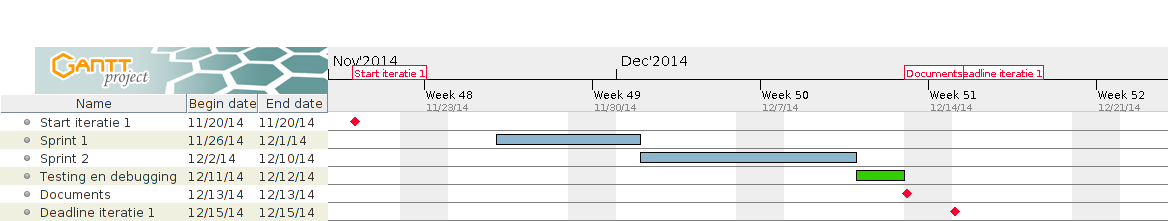
\includegraphics[width=1.2\linewidth]{./document.png}
\caption{Planning iteratie 1}
\label{fig:planning}
\end{figure}

  

\subsection{Evolutie van het SPMP}
De eerste versie van het SPMP wordt ingeleverd op 5 november 2014. Daarna zal bij elke iteratie een geüpdate versie van het SPMP worden meegegeven. De geschiedenis van het SPMP is gegeven in tabel \ref{tab:revchart}. De verantwoordelijkheid van dit document ligt bij de project manager. Dit SPMP volgt voornamelijk de standaard IEEE 1058-1998 \cite{ieeestd}.

\section{Referentiemateriaal}

\begin{thebibliography}{9}
\bibitem{ieeestd} \emph{IEEE Std 1058-1998}  
\bibitem{Website} \emph{Team Website} \url{http://wilma.vub.ac.be/~se2_1415/} \\
\bibitem{Wilma} \emph{Wilma} \url{http://wilma.vub.ac.be}\\
\bibitem{GitHub} \emph{GitHub Repository} \url{https://github.com/wiselib} \\
\bibitem{Teamwork} \emph{Teamwork} \url{https://wiselib.teamwork.com} \\
\bibitem{Slack} \emph{Slack} \url{https://wiselib.slack.com} \\
\bibitem{Sharelatex} \emph{ShareLa-eX} \url{https://www.sharelatex.com} \\

\bibitem{rvdstrae} \emph{Ragnhild Van Der Straeten} \href{mailto:rvdstrea@vub.ac.be}{rvdstrea@vub.ac.be} \\
\bibitem{jnicolay} \emph{Jens Nicolay} \href{mailto:jnicolay@vub.ac.be}{jnicolay@vub.ac.be} 
\bibitem{dvdeun} \emph{Dirk van Deun} \href{mailto:dirk@dinf.vub.ac.be}{dirk@dinf.vub.ac.be}
\end{thebibliography}

\section{Defenities en Acroniemen}

\begin{table}[h]
\centering
\begin{tabular}{c|c}
\textbf{Acroniem} & \textbf{Betekenis} \\
\hline
SPMP & Software Project Management Plan  \\
SRS & Software Requirements Specification \\
STP & Software Test Plan \\
SDD & Software Design Document \\
SQAP & Software Quality Assurance Plan \\
SCMP & Software Configuration Management Plan \\
VUB & Vrije Universiteit Brussel
\end{tabular}
\caption{Ancroniemen}
\label{tab:my_label}
\end{table}